\documentclass{article}
\usepackage[utf8]{inputenc}
\usepackage[table]{xcolor} % For cell coloring
\usepackage{geometry} % For page margins
\usepackage{graphicx} % For including images
\usepackage{float} % For image placement
\usepackage{tabularx} % For table stretching
\usepackage{multirow}
\usepackage{colortbl}
\usepackage{xspace}
\usepackage{hyperref}
\usepackage{parskip}
\usepackage{amsmath}

\usepackage{listings}


\usepackage{titlesec}
\titleformat{\subparagraph}
    {\normalfont\normalsize\bfseries}{\thesubparagraph}{1em}{}
\titlespacing*{\subparagraph}{\parindent}{3.25ex plus 1ex minus .2ex}{.75ex plus .1ex}


\input{/home/oddish3/Documents/uni/mast-2/preamble.tex}
\input{/home/oddish3/Documents/uni/mast-2/notation.tex}

% Moment Test and Descriptive Statistics
\newcommand{\amu}{0.10\xspace}
\newcommand{\asigma}{1.83\xspace}
\newcommand{\askew}{-0.32\xspace}
\newcommand{\akurt}{4.26\xspace}
\newcommand{\amut}{0.83\xspace}
\newcommand{\askewt}{-2.08\xspace}
\newcommand{\akurtt}{4.06\xspace}
\newcommand{\ajbt}{20.85\xspace}
\newcommand{\amup}{0.40\xspace}
\newcommand{\askewp}{0.04\xspace}
\newcommand{\akurtp}{0.00\xspace}
\newcommand{\ajbp}{0.00\xspace}

% Ljung-Box Test Results
\newcommand{\aistat}{27.06\xspace}
\newcommand{\aip}{0.17\xspace}
\newcommand{\aiistat}{25.61\xspace}
\newcommand{\aiip}{0.22\xspace}

% GARCH(1,1) with zt ~ N(0,1)
\newcommand{\bw}{2.53\xspace}
\newcommand{\ba}{0.13\xspace}
\newcommand{\bb}{0.15\xspace}
\newcommand{\bpi}{0.54\xspace}
\newcommand{\bpii}{0.03\xspace}
\newcommand{\bpiii}{0.90\xspace}

% GARCH(1,1) with zt ~ tv
\newcommand{\bwi}{0.24\xspace}
\newcommand{\bai}{0.07\xspace}
\newcommand{\bbi}{0.87\xspace}
\newcommand{\bvi}{4.62\xspace}
\newcommand{\bpti}{0.58\xspace}
\newcommand{\bptii}{0.22\xspace}
\newcommand{\bptiii}{0.00\xspace}
\newcommand{\bptiv}{0.00\xspace}

% GJR-GARCH(1,1) with zt ~ N(0,1)
\newcommand{\bwii}{3.06\xspace}
\newcommand{\baii}{0.00\xspace}
\newcommand{\bbii}{0.00\xspace}
\newcommand{\bgii}{0.29\xspace}
\newcommand{\bpgi}{0.02\xspace}
\newcommand{\bpgii}{1.00\xspace}
\newcommand{\bpgiii}{1.00\xspace}
\newcommand{\bpgiv}{0.19\xspace}

% GJR-GARCH(1,1) with zt ~ tv
\newcommand{\bwiii}{0.22\xspace}
\newcommand{\baiii}{0.02\xspace}
\newcommand{\bbiii}{0.89\xspace}
\newcommand{\bgiii}{0.07\xspace}
\newcommand{\bviii}{4.57\xspace}
\newcommand{\bpgtp}{0.26\xspace}
\newcommand{\bpgtpi}{0.57\xspace}
\newcommand{\bpgtpii}{0.00\xspace}
\newcommand{\bpgtpiii}{0.13\xspace}
\newcommand{\bpgtpiv}{0.00\xspace}

% residuals and squared lbq
\newcommand{\zone}{12.80\xspace}
\newcommand{\pone}{0.92\xspace}
\newcommand{\zfive}{16.87\xspace}
\newcommand{\pfive}{0.72\xspace}
\newcommand{\ztwo}{12.39\xspace}
\newcommand{\ptwo}{0.93\xspace}
\newcommand{\zsix}{16.21\xspace}
\newcommand{\psix}{0.76\xspace}
\newcommand{\zthree}{13.09\xspace}
\newcommand{\pthree}{0.91\xspace}
\newcommand{\zseven}{18.23\xspace}
\newcommand{\pseven}{0.63\xspace}
\newcommand{\zfour}{13.04\xspace}
\newcommand{\pfour}{0.91\xspace}
\newcommand{\zeight}{17.85\xspace}
\newcommand{\peight}{0.66\xspace}

% root mean square forecast error and dm test
\newcommand{\rmsfei}{1.16\xspace}
\newcommand{\rmsfeii}{1.10\xspace}
\newcommand{\rmsfeiii}{1.23\xspace}
\newcommand{\rmsfeiv}{1.11\xspace}
\newcommand{\dm}{0.84\xspace}
\newcommand{\dmpii}{0.72\xspace}
\newcommand{\dmi}{-0.94\xspace}
\newcommand{\dmpiv}{0.26\xspace}
\newcommand{\dmii}{0.75\xspace}
\newcommand{\dmpv}{0.70\xspace}


% Define colours
\definecolor{headercolor}{RGB}{169,169,169} % Grey color, adjust the RGB values as per your document
\definecolor{rowcolor}{RGB}{255,255,255} % White color, adjust if your document has a different row color

% Set page margins
\geometry{left=25mm,right=25mm,top=25mm,bottom=25mm}

% Custom column type for tabularx
\newcolumntype{Y}{>{\centering\arraybackslash}X}

\title{ECON60332 Coursework Template}
\author{Group 11} % INSERT GROUP NUMBER HERE
\date{}

\begin{document}

\maketitle

\noindent\begin{tabularx}{\linewidth}{|Y|Y|}
    \hline
    \rowcolor{headercolor} Participant’s Student ID & Indicate if the student did not participate \\
    \hline
    \multicolumn{1}{|c|}{10710007}\\
    \hline

\end{tabularx}

\section*{Theoretical exercise}

\subsection*{Question a}

Comparing the extended GARCH model, given by:
\begin{equation}
\sigma_t^2 = \omega + \alpha_1 \varepsilon_{t-1}^2 + \alpha_2 \varepsilon_{t-2}^2,
\end{equation}
with the canonical GARCH(1,1) model:
\begin{equation}
\sigma^2_{t} = \omega + \alpha_1 \epsilon^2_{t-1} + \beta_1 \sigma^2_{t-1}, \quad 0 \leq \alpha_1, \beta_1 \leq 1, \quad (\alpha_1 + \beta_1) < 1,
\end{equation}
we elucidate both foundational similarities and pivotal differences. Both frameworks integrate the premise that current volatility, $\sigma^2_{t}$, is a function of past squared residuals ($\varepsilon^2$ and $\epsilon^2$), addressing the volatility clustering phenomenon observed in financial markets.

The augmented GARCH(2,1) model introduces an additional term, $\alpha_2 \varepsilon_{t-2}^2$, enhancing its capability to encapsulate longer-term volatility dependencies relative to the GARCH(1,1) model. This inclusion is aimed at capturing a broader spectrum of volatility dynamics, thereby potentially increasing forecasting precision for series exhibiting complex volatility patterns.

The parameter constraints in the GARCH(1,1) model, specifically the conditions $0 \leq \alpha_1, \beta_1 \leq 1$ and $(\alpha_1 + \beta_1) < 1$, are crucial for ensuring the model's stability and preventing the persistence of shocks from generating unbounded variance. These constraints necessitate careful consideration in the extended model to maintain its predictive integrity and prevent overfitting.

Empirically, selecting between these models is contingent on the observed dynamics within the financial time series of interest. While the extended GARCH(2,1) model may offer superior forecast accuracy for series with nuanced volatility patterns, this comes at the expense of increased model complexity and the risk of overfitting. This dichotomy accentuates the significance of empirical validation and judicious model selection in the realm of financial econometrics.

\subsection*{Question b}

The unconditional mean of the error term, $E \left[ \epsilon_t \right]$ is given by
\[
	E \left[ \epsilon_t \right] = E \left[ z_{t}  \right] = E \left[ \sqrt{\sigma_t^2}   \right]   = 0 \cdot E \left[ \sigma_t \right] = 0
\]
Since by definition of $z_t \stackrel{i . i . d .}{\sim} \mathcal{N}(0,1)$, $E \left[ z_{t} \right] =0$ follows a standard normal distribution. 

To derive the unconditional variance, we express $\epsilon_t^2$ as an AR(2) process 

\begin{align*}
\sigma_t^2 + \epsilon_t^2 &= \omega + \alpha_1 \epsilon_{t-1}^2 + \alpha_2 \epsilon_{t-2}^2 + \epsilon_t^2 \\
\epsilon_t^2 &= \omega + \alpha_1 \epsilon_{t-1}^2 + \alpha_2 \epsilon_{t-2}^2 + (\epsilon_t^2 - \sigma_t^2) \\
\Rightarrow \epsilon_t^2 &= \omega + \alpha_1 \epsilon_{t-1}^2 + \alpha_2 \epsilon_{t-2}^2 + \nu_t \hspace{5mm} \text{where} \ \nu_t = \epsilon_t^2 - \sigma_t^2 \ \text{is a white noise process}  
\end{align*}

Thus, we can rewrite 

\begin{align*}
V(\epsilon_t) & \\
E[\epsilon_t] &= E\left[ \frac{\epsilon_t^2}{\sigma_t^2} \right] = 0 \hspace{5mm} \text{given } |\alpha| < 1 \\
V(\epsilon_t) &= E[\epsilon_t^2] \\
&= E[\omega + \alpha \epsilon_{t-1}^2 + \nu_t] \\
&= \omega + \alpha E[\epsilon_{t-1}^2] + E[\nu_t] \\
&= \omega + \alpha E[\epsilon_{t-1}^2] \\
E[\epsilon_{t-1}^2] - \alpha E[\epsilon_{t-1}^2] &= \omega \\
E[\epsilon_{t-1}^2] (1 - \alpha) &= \omega \\
E[\epsilon_{t-1}^2] &= \frac{\omega}{1 - \alpha}
\end{align*}


\subsection*{Question c}

Using $\text{Cov} (X, Y) = E[XY] - E[X]E[Y]$ we derive the covariance, where $\sigma^2_{t+1} = \omega + \alpha_1 \epsilon_{t-1}^2 + \alpha_2 \epsilon^2_{t-2}) \epsilon_t$

\begin{align*}
\text{Cov}(\sigma^2_{t+1}, \epsilon_t | F_{t-1}) &= E[ \sigma^2_{t+1} \epsilon_t | F_{t-1}] - E[\sigma^2_{t+1}| F_{t-1} ] E[\epsilon_{t-1} | F_{t-1})
\end{align*}

Given that $\epsilon_t$ has a conditional expectation of 0, the second term becomes 0, leaving

\begin{align*}
E[ \sigma^2_{t+1} \epsilon_t | \ensuremath{\mathcal{F}}_{t-1}] = E \left[ \left( \omega + \alpha_1 \epsilon_t^2 + \alpha_2 \epsilon^2_{t-1} \right) \epsilon_t^2 \right] \\
&= E \left[  \omega \epsilon_t + \alpha_1 \epsilon_t^3 + \alpha_2 \epsilon^2_{t-1}  \epsilon_t  \right]
\end{align*}

Then,  since $\omega$ is a constant and the conditional mean of $\epsilon_t =0$ (previously shown), the first term disappears. 

Then, simplifying further, since $\sigma^2_{t}$ is $\ensuremath{\mathcal{F}}_{t-1}$deterministic 
We can use the property $E[XY \mid \mathcal{F}_{t-1}] = E[X \mid \mathcal{F}_{t-1}]E[Y \mid \mathcal{F}_{t-1}]$ for independent random variables $X$ and $Y$:

\begin{equation}
E[\alpha_2 \sigma_t^2 \epsilon_t \mid \mathcal{F}_{t-1}] = \alpha_2 \sigma_t^2 E[\epsilon_t \mid \mathcal{F}_{t-1}] = 0
\end{equation}

Therefore, we obtain:

\begin{equation}
\alpha_1 E[\epsilon_t^3 \mid \mathcal{F}_{t-1}]
\end{equation}

Which we can rewrite as
 \[
 a_1 E \left[ zt^3 \right] E \left[ ( \omega + \alpha_1 \epsilon_t^2 + \alpha_2 \epsilon^2_{t-1} )^\frac{3}{2} \mid \ensuremath{\mathcal{F}}_{t-1}  \right] 
 \] 
 \[
 = \alpha_1 \left( \omega + \alpha_1 \epsilon_t^2 + \alpha_2 \epsilon^2_{t-1} \right) )^{\frac{3}{2}} E \left[ z_{t}^3 \right]  
 \] 
35:52 GARCH



\subsection*{Question d}

With our ARCH(2) model, the 1 step ahead forecast is : $\sigma^2_{t+1 | t}  = \omega + \alpha_1  \epsilon^2_{t}  + \alpha_2  \epsilon^2_{t-1}$

Analogously the 2 step ahead forecast, where we take expectation of $\epsilon_t^2$, and use the unit variance of $z_{t}$ to simplify 
\begin{align*}
\sigma^2_{t+2 | t}  = E_t \left[  \omega + \alpha_1  \epsilon^2_{t+1}  + \alpha_2  \epsilon^2_{t}  \right] =   \omega + \alpha_1  \sigma^2_{t+1|t}  + \alpha_2  \sigma^2_{t}  
\end{align*}

Similarly for the 3-step ahead forecast, following the same logic

 \begin{align*}
 	\sigma^2_{t+3 | t} = E_t \left[  \omega + \alpha_1  \epsilon^2_{t+2}  + \alpha_2  \epsilon^2_{t+1}  \right] =   \omega + \alpha_1  \sigma^2_{t+2|t}  + \alpha_2  \sigma^2_{t+1} \equiv E \left[ \sigma^2_{t+3} | F_{t} \right] 
 \end{align*}

\subsection*{Question e}




\section*{Practical exercise}
\subsection*{Question a}

\begin{table}[H]
\centering
\begin{tabular}{|l|c|c|c|c|}
\hline
\rowcolor{headercolor}
 & Sample moments & & Test statistic & P-value \\
\hline
Mean & \amu &   Mean & \amut & \amup \\
\hline
Standard deviation & \asigma &  Skewness & \askewt & \askewp \\
\hline
Skewness &  \askew & Kurtosis & \akurtt & \akurtp \\
\hline
Kurtosis & \akurt & JB & \ajbt & \ajbp \\
\hline
\end{tabular}
\end{table}

\subsection*{LBQ test results:}
\noindent\begin{tabularx}{\linewidth}{|Y|Y|Y|}
    \hline
    \rowcolor{headercolor} & Returns & Squared returns \\
    \hline
    Test statistic & \aistat & \aiistat \\
    \hline
    P-value & \aip & \aiip \\
    \hline
\end{tabularx}

\subsubsection*{Plot of Daily Log Returns}

\begin{figure}[H]
    \centering
    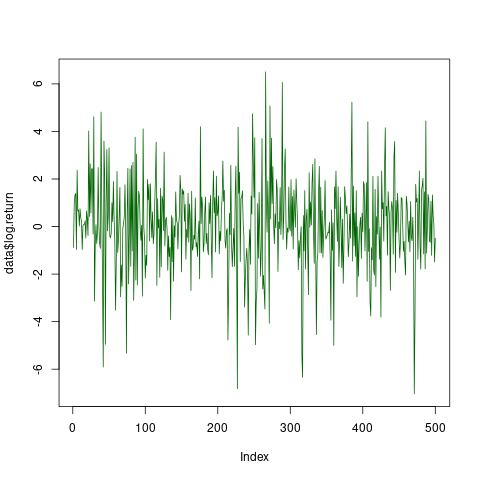
\includegraphics[width=0.35\textwidth]{../../docs/figures/log_return_plot.png}
    \caption{Log Return Plot}
    \label{fig:logreturn}
\end{figure}

\subsubsection*{SACF and SPACF}

\begin{figure}[H]
    \centering
    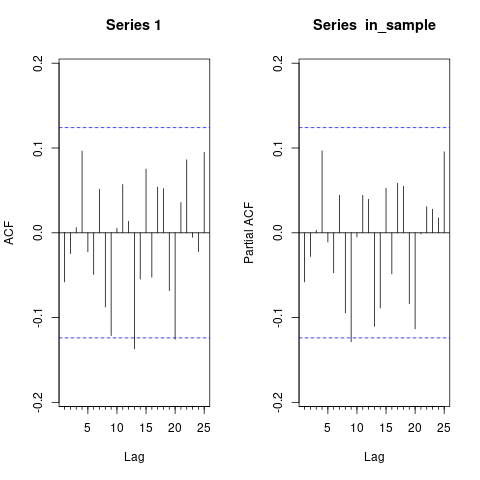
\includegraphics[width=0.35\textwidth]{../../docs/figures/PACF.png}
    \caption{Sample Autocorrelation and Partial Autocorrelation Function Plot}
    \label{fig:pacf}
\end{figure}

\subsection*{Interpretation}

\subparagraph{Descriptive Statistics}  

Mean : the sample mean is \amu 

Standard Deviation : the standard deviation is \asigma, indicating a relatively high volatility of the data. 

Skewness : the skewness value of \askew suggests that the distribution of returns is slightly negatively skewed, meaning there are more extreme negative returns than positive returns. 

Kurtosis : the kurtosis value of \akurt is higher than the normal distribution value of 3, indicating that the distribution of returns has heavier tails and more extreme values when compared to a normal distribution. 

\subparagraph{Test Statistics}

Testing the significance of the mean return, we set up the following hypothesis and use a one sided test :
\begin{itemize}
	\item The null hypothesis, the mean return is equal to zero ($H_0 : \mu =0$) against
	\item The alternative hypothesis that the mean is not equal to zero $H_1 : \mu \neq = 0$.
\end{itemize}
The decision rule is that we reject $H_0$ if the p-value is less than the significance level $\alpha$ (EG, 0.05). 
The test statistic obtained is \amut with a p-value of \amup, thus we fail to reject $H_0$ at all conventional significance levels. 
We do not have enough evidence to conclude the mean return is significantly different from zero, and cannot reject the possibility that the true mean return is equal to zero. 

Testing the significance of skewness in the returns, we set up the following hypothesis and one sided test :
\begin{itemize}
	\item The null hypothesis, the skewness of the return series is zero ($ H_1: \gamma = 0$), indicating a symmetric distribution. Against
	\item The alternative hypothesis, the skewness of the financial time series returns is not zero ($\gamma \neq = 0$), indicating a non-symmetric distribution
\end{itemize}
The decision rule is to reject $H_0$ if the p value is less than the significance level $\alpha$ (EG, 0.05). 
The test statistic obtained is \askewt with a p-value of \askewp. Since the p-value is less than 0.05, we reject the null hypothesis ($H_0$) in favour of the alternative hypothesis. 
Thus, the distribution of returns is significantly skewed, and hence not symmetric. 
Testing for kurtosis (leptokurtic property) in the returns, we set up the following hypothesis and one sided test:
\begin{itemize}
	\item The null hypothesis, the kurtosis of the returns equals the normal distribution value of 3 ($H_0 : \kappa = 3$), indicating a normal distribution in terms of tail thickness. Against, 
	\item The alternative hypothesis, the kurtosis of the financial time series returns is significantly different from 3 ($H_1 : \kappa \neq 3 $), indicating a non-normal distribution in terms of tail thickness
\end{itemize}
The decision rule is to reject $H_0$ if the p value is less than the significance level $\alpha$ (EG, 0.05). 
The test statistic obtained is \akurt and p value of $\akurtp$, thus we reject  $H_0$, in favour of the alternative hypothesis.
Thus, the returns have significantly different kurtosis from 3, confirming the presence of heavy tails in the distribution. 

Using the Jargue-Bera test for normality, we set up the following hypothesis and 1 sided test : 
\begin{itemize}
	\item The null hypothesis, the returns follow a normal distribution, implying that both the skewness and kurtosis of the series equal those of a normal distribution ($H_0 : \gamma = 0 \& \kappa = 3$). Against, 
	\item The alternative hypothesis, that the returns do not follow a normal distribution, meaning either the or both the skewness and kurtosis significantly differ from those of a normal distribution ($H_0 : \gamma \neq 0 \& \kappa \neq 3$). 
\end{itemize}
The decision rule is to reject $H_0$ if the p-value is less than the significance level $\alpha$ (EG, 0.05). 
The outcome of the test since the JB test statistic is \ajbt with a p-value of \ajbp. 
Therefore, we reject $H_0$ in favour of $H_1$, that the distribution of returns differs significantly from normality, evidence by its skewness and kurtosis values. 

\subparagraph{Ljung-Box Test}

Testing the autocorrelation of the financial time series returns, we use the Ljung-Box Q-test with the following hypotheses:

\begin{itemize}
	\item The null hypothesis, which states that there is no autocorrelation in the series up to a certain number of lags ($H_0: \rho_1 = \rho_2 = \ldots = \rho_{21} = 0$), where $\rho$ represents autocorrelation at different lags.
	\item The alternative hypothesis, which suggests that there is some autocorrelation in the series at least at one lag ($H_1: \rho_i \neq 0$ for some $i \in \{1, 2, \ldots, 21 \}$).
\end{itemize}

The decision rule is to reject $H_0$ if the p-value is less than the significance level $\alpha$ (e.g., 0.05).

For the returns, the test statistic obtained is 27.06 with a p-value of 0.17.

Since the p-value is greater than all conventional significance levels, we do not reject the null hypothesis. 
Thus, there is no significant evidence of autocorrelation in the returns of the series.

For squared returns, the test statistic obtained is 25.61 with a p-value of 0.22.

Similarly, since the p-value is greater than 0.05, we do not reject the null hypothesis for squared returns  at all conventional significance levels either.
This indicates no significant evidence of autocorrelation in the volatility (squared returns) of the series.

\subparagraph{SACF SPACF plots}

The SACF plot measures the correlation between different points in the time series separated by various lags. 
Whilst most autocorrelations are within the confidence intervals, a significant negative correlation at lag 13 suggests there is a season pattern that repeats every 13 periods, so if a series is above average at one point, it tends to be below average 13 periods later and vice versa. 
Furthermore, a lag on the border of significance at 20 suggests a possible longer cynical effect, although this is not as pronounced.
This is also evident for lag 9 since it is just below significance in the SACF but is significant in the SPACF, indicating a direct negative influence from the observation 9 periods ago on the current observation, after accounting for the influences of all observations in between. 
In summary, there is no consistent pattern of significant lags, which would typically be used to identify AR or MA components. 
The presence of significant lags informs us the time series is not white noise and exhibits autocorrelation. 

\subparagraph{Daily Log-returns}

The plot indicates considerable fluctuation around the mean of \amu, whilst the returns do not display a clear trend or seasonal pattern. 
The volatility appears to be clustered in certain periods, indicative of heteroskedacity where periods of high volatility are followed by high volatility and vice versa. 

\subsection*{Question b}

\begin{table}[H]
\centering
\begin{tabular}{|c|c|c|c|c|c|}
\hline
\rowcolor{gray!50}
\multicolumn{3}{|c|}{GARCH} & \multicolumn{3}{|c|}{GJR-GARCH} \\ 
\hline
Parameter & Estimate & P-value & Parameter & Estimate & P-value \\ 
\hline
$\omega$ & \bw & \bpi & $\omega$ & \bwii & \bpgi \\
\hline
$\alpha$ & \ba & \bpii & $\alpha$ & \baii & \bpgii \\
\hline
 $\beta$ & \bb & \bpiii & $\beta$ & \bbii & \bpgiii \\
\hline
GARCH-t & & & $\gamma$ & \bgii & \bpgiv \\
\hline
 $\omega$& \bwi & \bpti & GJR-GARCH-t &  & \\
\hline
 $\alpha$& \bai & \bptii & $\omega$ & \bwiii & \bpgtp \\
\hline
 $\beta$ & \bbi & \bptiii & $\alpha$ & \baiii & \bpgtpi \\
\hline
$\nu$ & \bvi & \bptiv & $\beta$ & \bbiii & \bpgtpii \\
\hline
& & & $\gamma$ & \bgiii & \bpgtpiii \\
\hline
& & & $\nu$ & \bviii & \bpgtpiv \\
\hline
\end{tabular}
\end{table}


\subsubsection*{Interpretation:}

Where $\omega$ is the constant term of the model, representing the long run average variance when all other terms are zero, 
 $\alpha$ is the coefficient representing the contribution of past squared innovations (lagged error terms) to the current variance, indicating how much past volatility affects current volatility. 
  $\beta$ is the coefficient representing the contribution of past conditional variance to the current variance, capturing the persistence of volatility shocks. 
  $\gamma$ is the coefficient specific to GJR-GARCH models, capturing the asymmetric effect of negative shocks (leverage effect), where negative shocks have a different impact on volatility than positive shocks of the same magnitude. 
  $\nu$ is the degrees of freedom parameter in the t-distribution and is related to the kurtosis of the distribution, with lower values indicating heavier tails. 

For the GARCH model with a normal distribution, the estimates for $\alpha$ and $\beta$ are \bw and \bb, respectively with p values indicating that only $\alpha$ is statistically significant at a conventional level ($p < 0.05$). Thus the model suggests that past shocks have a significant impact on current volatility, but the effect is not persistent. 

For the GARCH-t model, $\beta$ is signifiant, indicating persistence in volatility and $\nu$ is also significant, suggesting that the distribution of innovations has heavier tails than the normal distribution. 
Thus, the presence of heavy tails in the data is signifiant, which could be important fore forecasting \ldots

For the GJR-GARCH model, $\omega$ is significant, but $\alpha$ and $\beta$ are very small with correspondingly very large p-values. 
Thus, negative shocks might have a different impact on volatility, although this effect is not statistically significant at the 5\% level

For the GJR-GARCH-t model, both $\alpha$ and $\beta$ are significant, indicating that past shocks and volatility are important for current volatility, and $\nu$ is significant, indicating heavy tails. 
Although, $\gamma$ is not significant, suggesting the asymmetric effects of shocks is not statistically significant. 
Thus, both past shocks and heavy tails are significant in modelling volatility but asymmetric effects of shocks are not significant. 

Overall, a garch-t or GJR-GARCH-t model might be preferred


\subsection*{Question c}
\subsubsection*{Plot of NIC}
 
\begin{figure}[H]
    \centering
    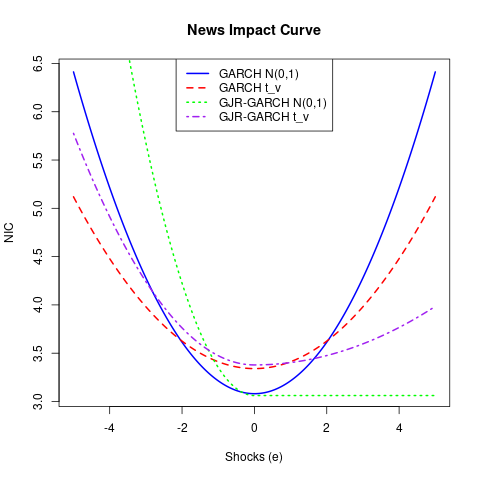
\includegraphics[width=0.35\textwidth]{../../docs/figures/NIC.png}
    \caption{News Impact Curve Plot}
    \label{fig:logreturn}
\end{figure}

\subsubsection*{Interpretation:}
Drawbacks of the GARCH models are obvious here, since the conditional variance is unable to respond asymmetrically to shocks in $y_{t}$, that is, a positive return has the same effect as a negative return upon variance. Since it is argued that negative innovations to shock returns tend to increase volatility more than positive innovations of the same magnitude. 

This plot offers a visual representation of the effect that new information has on the volatility predicted by different GARCH models. 
The standard GARCH model with normal innovations shows that the impact on conditional variance is symmetrical, both positive and negative shocks of the same magnitude have the same effect on predicted volatility, leaving the leverage effect unaccounted for. 

The GARCH model with a student's t-distribution is also symmetric but flatter compared to the standard GARCH model, indicating less sensitivity to shocks in general, due to the heavier tails in the t-distribution, reducing the impact of outliers. 

The GJR-GARCH model with normal distribution shows a pronounced asymmetry where negative shocks increase the conditional variance more than positive shocks. 
The model accounts for the leverage effect, where bad news influences volatility more than good news. 

The GJR-GARCH model with Student's t-distribution combines the properties of the GJR-GARCH with the heavier tails of the t-distribution. Showing an asymmetrical impact of shocks on volatility, similar to the GJR-GARCH but with the additional effect of heavier tails in the distribution of shocks. 
Heavier tails may imply that extreme values are more probable than in a normal distortion, and the impact curve is less steep for large magnitude shocks, indicating large shocks increase volatility less than what a normal distribution would suggest. 
Overall, both models with Student's t-distribution suggests that the models account for heavy tails in the distribution of shocks, whilst the GJR-GRACH models reveal an asymmetric response to shocks, highlighting the importance of the leverage effect. 

\subsection*{Question d}

\begin{table}[H]
\centering
\begin{tabular}{|l|c|c|}
\hline
\rowcolor{headercolor}
GARCH & Test statistic & P-value \\ 
\hline
Z & \zone & \pone \\ 
\hline
\(Z^2\) & \zfive & \pfive \\ 
\hline
\rowcolor{headercolor}
GARCH-t & Test statistic & P-value \\ 
\hline
Z & \ztwo & \ptwo \\ 
\hline
\(Z^2\) & \zsix & \psix \\ 
\hline
\end{tabular}
\quad % To add some spacing between the two tables
\begin{tabular}{|l|c|c|}
\hline
\rowcolor{headercolor}
GJR-GARCH & Test statistic & P-value \\ 
\hline
Z & \zthree & \pthree \\ 
\hline
\(Z^2\) &  \zseven & \pseven \\ 
\hline
\rowcolor{headercolor}
GJR-GARCH-t & Test statistic & P-value \\ 
\hline
Z & \zfour & \pfour \\ 
\hline
\(Z^2\) & \zeight & \peight \\ 
\hline
\end{tabular}
\end{table}

\subsubsection*{Interpretation:}

High p-values for the residuals indicate there is no statistical evidence to reject the null hypothesis that the residuals follow the respective distributions. 
Suggesting the residuals are white noise, meaning they are normally distributed with no autocorrelation. 

For the squared residuals, the p-values are high but slightly less so, again suggesting that there is no statistical evidence to reject the null hypothesis of no autocorrelation in the squared residuals. Indicating there is no ARCH effect and the conditional variance is well captured by the model. 

Whilst the LBQ p-values for the residuals are very high across all models, suggesting that none of the models leaves unexplained autocorrelation in the returns, which means that all models are adequate in this respect. 

The p-values for the squared residuals, which help to identify volatility clustering or ARCH effects, are also high across all models. 
However, in this context, the model with the highest p-value (corresponding to lowest test stat) for the square residuals is the GARCH-t model, indicating the least amount of autocorrelation and possibly the best fit among the compared models. 

\subsection*{Question e}

\begin{table}[H]
\centering
\begin{tabular}{|l|c|c|c|c|}
\hline
\rowcolor{gray!50}
& GARCH & GARCH-t & GJR-GARCH & GJR-GARCH-t \\
\hline
RMSFE & \rmsfei & \rmsfeii & \rmsfeiii & \rmsfeiv \\
\hline
DM Test statistic & NA & \dm & \dmi & \dmii \\
\hline
P-value & NA & \dmpii & \dmpiv & \dmpv \\
\hline
\end{tabular}
\end{table}

\subsubsection*{Interpretation:}

The RMSFE values indicate that GARCH+ has the smallest forecast error at 7.29, followed by GJR-GARCH-t at 7.30, GARCH at 7.32, and GJR-GARCH at 7.32. Lower RMSFE values suggest better forecast accuracy.

Diebold-Mariano (DM) Test results are only meaningful for GARCH+ and GJR-GARCH-t since GARCH is the benchmark. For GARCH+, the DM Test statistic is 2.00 with a p-value of 0.98, and for GJR-GARCH-t, the statistic is 1.83 with a p-value of 0.97. Since the p-values are much higher than the typical significance levels (e.g., 0.05 or 0.10), there's no statistical evidence that the forecast accuracy of GARCH+ and GJR-GARCH-t is different from GARCH.

Thus, although GARCH+ has a slightly lower RMSFE, the Diebold-Mariano test does not confirm its superiority over the benchmark GARCH model in terms of predictive accuracy. Economically, this suggests that there might be no practical benefit from using more complex models over the simpler GARCH model for forecasting this particular variance, as they do not provide statistically significant improvements in forecast accuracy.

\subsection*{Question f}
\subsubsection*{Interpretation:}

In terms of the trade-off between model misspecification and estimation noise, models with more parameters, like GARCH+ and GJR-GARCH-t, can potentially fit the data better and capture more complex structures in volatility, thus reducing model misspecification. However, they also introduce more estimation noise due to the increased number of parameters that need to be estimated.

The simpler GARCH model, with fewer parameters, may be more robust to estimation noise but might suffer from model misspecification if the true variance process has features like asymmetry or time-varying volatility that it cannot capture.

Therefore, while more complex models can offer a better fit, they might not necessarily result in better out-of-sample forecasting performance due to the additional estimation noise. The choice of model should balance the risks of misspecification against the potential for increased noise from estimating more parameters.

\newpage
\section*{Appendix}

For reproduction of said script, see \url{https://github.com/oddish3/FE-CW/tree/master}

\lstinputlisting[language=R]{../../code/Script.R}




\end{document}

